\section{Aeropuertos}
En la gran nación de Pythonia tienen una vasta de red de aeropuertos y aviones, la cual utiliza una gran base de datos y computadores cuánticos para funcionar. Lamentablemente, como es común en Pythonia, los algoritmos implementados resultaron insuficientes para manejar el constante progreso de la nación, por lo que solicitaron ayuda de los alumnos de programación de la Universidad Santa Maria.\\\\
Los actuales gerentes de aeropuertos de la nación nos informan que almacenan la mayoría de sus datos en archivos, donde tienen un archivo para todos los aeropuertos llamado \texttt{Aeropuertos.txt}, donde se almacenan el id del aeropuerto, su ubicación, su cantidad de pistas, su tamaño y el código de su gerente. También, nos cuentan que para cada día ellos tienen un archivo \texttt{Vuelos\_dia\_mes\_año} donde \texttt{dia,mes} y \texttt{año} son la fecha asociada al archivo (considere que existen archivos para todas las fechas posibles).
\\
\\
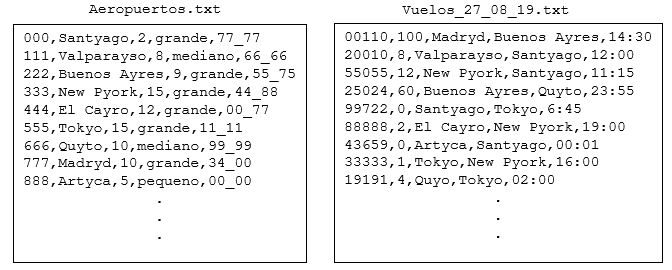
\includegraphics[scale=0.9]{Imagenes/original.PNG}\\\\
Se le solicita que implemente las siguientes funciones:
\begin{itemize}
    \item \texttt{cantidad\_recibidos(arch\_aeropuertos, fecha\_vuelos)} la cual recibe el nombre del archivo de aeropuertos y la fecha a verificar, la función debe retornar un diccionario, donde la llave es el nombre del aeropuerto y su valor la cantidad de vuelos que arriban a ese aeropuerto en la fecha \texttt{fecha\_vuelos}, la cual vendrá de formato \texttt{dia-mes-año}. Si un areopuerto no recibe vuelos ese día, no debe mostrarse en el diccionario.
\begin{lstlisting}[style=consola]
>>> [*cantidad_recibidos('Aeropuertos.txt','27-08-2019')*]
{'Buenos Ayres': 1, 'Santyago': 3, 'Quyto': 1, 'Tokyo': 2, 'New Pyork': 2}
\end{lstlisting}
    \item \texttt{verificar\_pistas(arch\_aeropuertos, fecha\_vuelos)} la cual verifica para todos los aeropuertos, si la cantidad de vuelos que les llega en el dia \texttt{fecha\_vuelos} supera o no las pistas que este posee. La función debe retornar \texttt{True} en caso de que no existan irregularidades, para el caso contrario, debe retornar una lista de las ciudades con este conflicto.
\begin{lstlisting}[style=consola]
>>> [*verificar_pistas('Aeropuertos.txt','27-08-2019')*]
['Santyago']
\end{lstlisting}
\item \texttt{agregar\_aeropuerto(arch\_aeropuertos,id\_a,nombre,pistas,tamano,gerente)} la cual escribe en el archivo de aeropuertos el nuevo aeropuerto a ingresar, note que el archivo esta ordenado por las ID's de menor a mayor, por lo que debe mantenerse así. En caso de que el \texttt{id\_a} del aeropuerto entregado ya esté en el archivo, la función debe retornar \texttt{False}, si se ingresó con éxito, debe retornar \texttt{True}. Asuma que los rut de gerentes pueden repetirse.
\begin{lstlisting}[style=consola]
>>> [*agregar_aeropuerto('Aeropuertos.txt','27-08-2019',800,'Parys',
10,'mediano','55_55')*]
True
\end{lstlisting}
\begin{center}
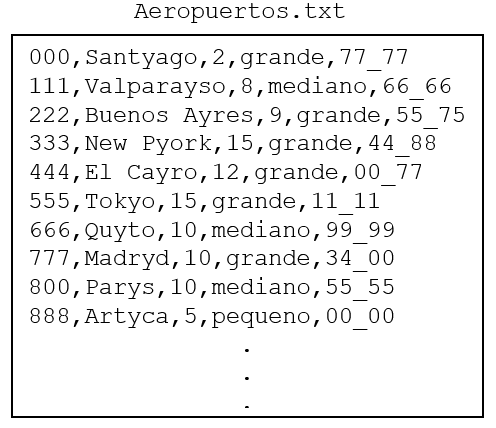
\includegraphics[scale=0.6]{Imagenes/nuevo.PNG}
\end{center}
\end{itemize}
\subsection{Desafíos \textit{(opcional)}}
\begin{itemize}
    \item Implemente \texttt{cantidad\_recibidos()} sin utilizar \texttt{arch\_aeropuertos}
    \item Implemente \texttt{verificar\_pistas()} sin utilizar listas (sin contar la necesaria al retornar)
    \item Implemente \texttt{agregar\_aeropuerto()} sin utilizar ninguna vez el método \texttt{sort()}.
\end{itemize}
Si lograste programar bajo los desafíos (o los realizaste sin querer), Felicidades!, Pyñera estará orgulloso.


\section{Espías}
Después de su impecable implementación en los aeropuertos, las organizaciones de seguridad han detectado espías malvados de la nación de Javalonia inflitrados como gerentes falsos de aeropuertos. Lograron identificar que, los ruts de los gerentes espías tienen la particularidad de que su formato no sigue la forma \texttt{XX\_YY}, tal que si un par (separado por \_) no tiene los mismos números, es un espía de Javalonia.\\\\
Para esto, se le solicita implementar la función \texttt{eliminar\_espias(arch\_aeropuerto)}, la cual modifica el archivo de aeropuertos, reemplazando el rut conflictivo con los caracteres \texttt{XX\_XX}. La función debe retornar un diccionario con llaves los aeropuertos afectados y su valor respectivo el rut del espia encontrado, o \texttt{False} si no se modificó el archivo. 
\begin{lstlisting}[style=consola]
>>> [*eliminar_espias('Aeropuertos.txt')*]
{'Buenos Ayres':'55_75', 'Madryd':'34_00'}
\end{lstlisting}
\begin{center}
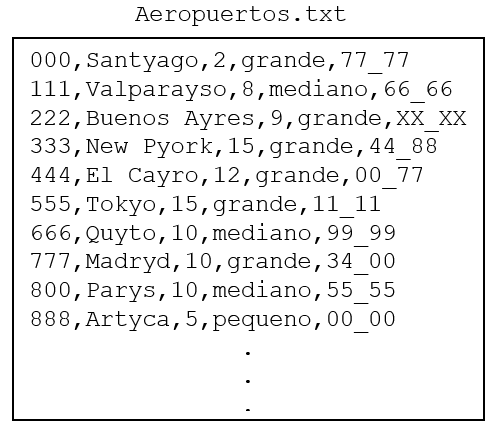
\includegraphics[scale=0.6]{Imagenes/espias.PNG}
\end{center}
\section{Legado}
Sus implementaciones hicieron eco en toda la nación de Pythonia, y los estudiantes novatos de programación decidieron acudir a ustedes para recibir consejos acerca de sus códigos. A continuación se le mostraráalgunos de los códigos de ellos, junto con qué es lo que debería hacer, lo cual debido a un error lógico o semántico (una lógica incorrecta o mal llamado a función) no funciona. Su labor es escribir una respuesta que le haga entender qué es lo que falló y como resolverlo (puede ser en texto o en un ejemplo, pero se recomienda expresarse en palabras )
\begin{itemize}
    \item Se busca aumentar en uno a todos los números de un archivo (donde existe sólo un número por linea).
  \begin{lstlisting}[style=consola]
arch = open("Numeros.txt")
for linea in arch:
    linea=int(linea.strip())
    arch.write(str(linea+1))
arch.close()
\end{lstlisting}
\textit{``Quiero escribir el número que me encuentre pero aumentándolo en uno, sin embargo el código no parece escribir en el archivo"}
\end{itemize}
\begin{center}

\includegraphics[width=0.9\textwidth]{Imagenes/blanco.PNG}
\end{center}
\newpage
\begin{itemize}
    \item La función \texttt{maximo} debe retornar la llave con mayor valor del diccionario entregado (el diccionario tiene números \texttt{int} como llaves).
  \begin{lstlisting}[style=consola]
def maximo(dicc):
    print(max(dicc.keys()))
\end{lstlisting}
\textit{``Utilizo esta función dentro de mi código principal, pero al llamarla me quedan variables sin valor"}
\end{itemize}
\begin{center}

\includegraphics[width=0.9\textwidth]{Imagenes/blanco.PNG}
\end{center}

\begin{itemize}
    \item Piden crear una funcion \texttt{apellido(dicc,nom)}, donde para un diccionario de formato \texttt{\{nombre:apellido\}} se busque el apellido asociado a \texttt{nom}.
  \begin{lstlisting}[style=consola]
def apellido(dicc,nom):
    for nombre,apellido in dicc.items:
        if nombre == nom:
            return apellido
\end{lstlisting}
    \textit{``Busco recorrer el diccionario hasta encontrar el nombre, porque yo se que estará asociado a su apellido, pero el código me arroja un error que no puedo entender:"} \texttt{TypeError: 'builtin\_function\_or \_method' object is not iterable}
\end{itemize}
\begin{center}
 
\includegraphics[width=0.9\textwidth]{Imagenes/blanco.PNG}   
\end{center}
\section{Encuesta final}
Para apoyar a su querido ayudante, por favor responda esta rápida encuesta: \texttt{bit.ly/30GtdnG} 
\begin{center}

\includegraphics[width=0.3\textwidth]{Imagenes/QR.PNG}
\end{center}



